\documentclass[12pt]{article}
\usepackage{fontspec}
\usepackage{fullpage}
\usepackage{hyperref}
\hypersetup{bookmarks=true,colorlinks=true,linkcolor=red,citecolor=blue,filecolor=magenta,urlcolor=cyan}
\usepackage{amsmath}
\usepackage{amssymb}
\usepackage{mathtools}
\usepackage{unicode-math}
\usepackage{tabu}
\usepackage{longtable}
\usepackage{booktabs}
\usepackage{caption}
\usepackage{enumitem}
\usepackage{graphics}
\usepackage{filecontents}
\usepackage[backend=bibtex]{biblatex}
\usepackage{url}
\setmathfont{Latin Modern Math}
\newcommand{\gt}{\ensuremath >}
\newcommand{\lt}{\ensuremath <}
\global\tabulinesep=1mm
\newlist{symbDescription}{description}{1}
\setlist[symbDescription]{noitemsep, topsep=0pt, parsep=0pt, partopsep=0pt}
\bibliography{bibfile}
\title{Software Requirements Specification for Diagnose}
\author{Andrea Clemeno}
\begin{document}
\maketitle
\tableofcontents
\newpage
\section{Reference Material}
\label{Sec:RefMat}
This section records information for easy reference.

\subsection{Table of Units}
\label{Sec:ToU}
The unit system used throughout is SI (Système International d'Unités). In addition to the basic units, several derived units are also used. For each unit, \hyperref[Table:ToU]{Tab: ToU} lists the symbol, a description and the SI name.

\begin{longtable}{l l l}
\toprule
\textbf{Symbol} & \textbf{Description} & \textbf{SI Name}
\\
\midrule
\endhead
${\text{d}}$ & time & day
\\
${\text{mL}}$ & volume & millilitre
\\
${\text{mol}}$ & amount of substance & mole
\\
\bottomrule
\caption{Table of Units}
\label{Table:ToU}
\end{longtable}
\subsection{Table of Symbols}
\label{Sec:ToS}
The symbols used in this document are summarized in \hyperref[Table:ToS]{Tab: ToS} along with their units. Throughout the document, symbols in bold will represent vectors, and scalars otherwise. The symbols are listed in alphabetical order. For vector quantities, the units shown are for each component of the vector.

\begin{longtable}{l l l}
\toprule
\textbf{Symbol} & \textbf{Description} & \textbf{Units}
\\
\midrule
\endhead
$k$ & Elimination constant & $\text{d}^{-1}$
\\
$N$ & Viral load & $\frac{\text{mol}}{\text{mL}}$
\\
${N_{\text{o}}}$ & Initial viral load & $\frac{\text{mol}}{\text{mL}}$
\\
${N_{\text{p}}}$ & Predicted viral load after 30 days & $\frac{\text{mol}}{\text{mL}}$
\\
${N_{\text{t}}}$ & Viral load at time t & $\frac{\text{mol}}{\text{mL}}$
\\
$n$ & Number of virions & ${\text{mol}}$
\\
$r$ & Rate of change of the viral load & $\frac{\text{mol}}{\text{mL}\text{d}}$
\\
$t$ & Time & ${\text{d}}$
\\
${t_{\text{p}}}$ & Chosen prediction period & ${\text{d}}$
\\
${t_{\text{t}}}$ & Time at secondary test & ${\text{d}}$
\\
$V$ & Volume & ${\text{mL}}$
\\
\bottomrule
\caption{Table of Symbols}
\label{Table:ToS}
\end{longtable}
\subsection{Abbreviations and Acronyms}
\label{Sec:TAbbAcc}
\begin{longtable}{l l}
\toprule
\textbf{Abbreviation} & \textbf{Full Form}
\\
\midrule
\endhead
A & Assumption
\\
DD & Data Definition
\\
GD & General Definition
\\
GS & Goal Statement
\\
IM & Instance Model
\\
PS & Physical System Description
\\
R & Requirement
\\
SRS & Software Requirements Specification
\\
TM & Theoretical Model
\\
Uncert. & Typical Uncertainty
\\
\bottomrule
\caption{Abbreviations and Acronyms}
\label{Table:TAbbAcc}
\end{longtable}
\section{Introduction}
\label{Sec:Intro}
HIV-1 is a virus that attacks cells of the immune system needed to fight off diseases. The virus leads to an uncurable disease called AIDs. Therefore, it is useful to have a program to model these types of problems. The program documented here is called Diagnose.

The following section provides an overview of the Software Requirements Specification (SRS) for Diagnose. This section explains the purpose of this document, the scope of the requirements, the characteristics of the intended reader, and the organization of the document.

\subsection{Scope of Requirements}
\label{Sec:ReqsScope}
The scope of the requirements includes the analysis of HIV-1 concentration over time.

\section{Specific System Description}
\label{Sec:SpecSystDesc}
This section first presents the problem description, which gives a high-level view of the problem to be solved. This is followed by the solution characteristics specification, which presents the assumptions, theories, and definitions that are used.

\subsection{Problem Description}
\label{Sec:ProbDesc}
A system is needed to assess the risk before substantial immune destruction has occurred. The system will predict viral load at 30 days and the patient's progression.

\subsubsection{Terminology and Definitions}
\label{Sec:TermDefs}
This subsection provides a list of terms that are used in the subsequent sections and their meaning, with the purpose of reducing ambiguity and making it easier to correctly understand the requirements.

\begin{itemize}
\item{Virus: Submicroscopic parasites that infect cells.}
\item{Viral load: The concentration of HIV virus at a point in time.}
\item{Infected cells: Cells that interact with the virus replicate into cells altered by the virus.}
\item{Helper T cell: Cells of the immune system that neutralize infected cells.}
\item{Elimination: Physical quantity undergoing a decline in amount.}
\item{AIDs: Acquired Immunodeficiency Syndrome develops from an increase in HIV viral load to the extent where T cell count decreases to under 200 mol/L.}
\item{Diagnosis: The determination of a patient's condition reached by a healthcare professional.}
\item{Progression: The development towards a more advanced stage.}
\end{itemize}
\subsubsection{Physical System Description}
\label{Sec:PhysSyst}
The physical system of Diagnose, as shown in \hyperref[Figure:Virus]{Fig:Virus}, includes the following elements:

\begin{itemize}
\item[PS1:]{The HIV Virion.}
\item[PS2:]{The virus-infected cells.}
\item[PS3:]{The Helper T cell.}
\item[PS4:]{The Human Body.}
\end{itemize}
\begin{figure}
\begin{center}
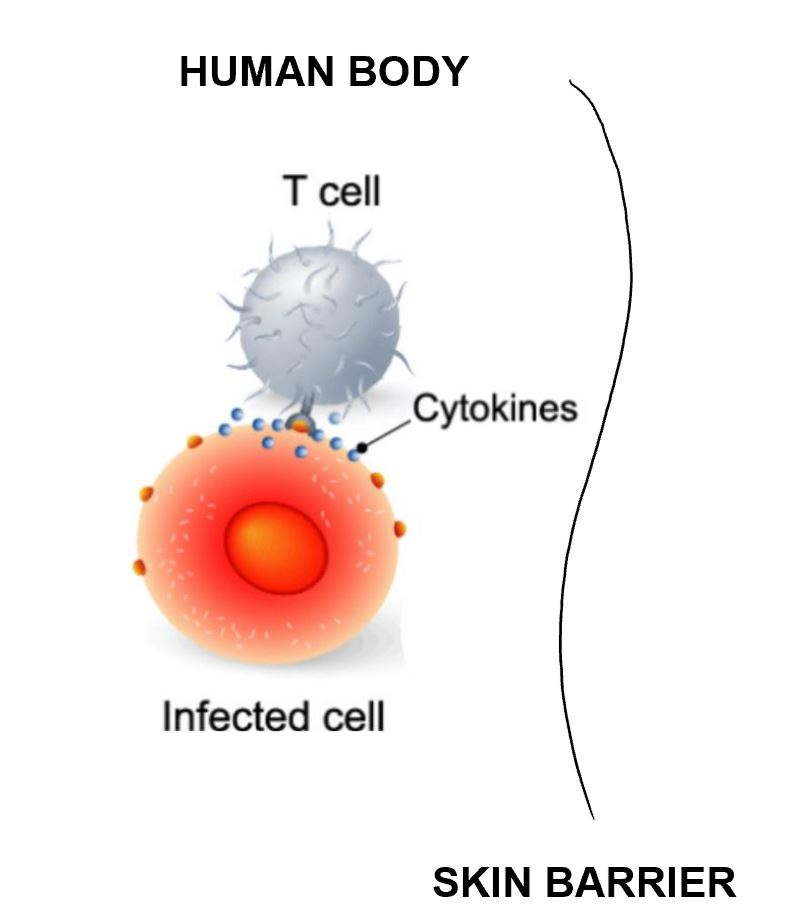
\includegraphics[width=0.7\textwidth]{../../../datafiles/Diagnose/Virusinbody.JPG}
\caption{The physical system}
\label{Figure:Virus}
\end{center}
\end{figure}
\subsubsection{Goal Statements}
\label{Sec:GoalStmt}
Given two HIV-1 viral load datum taken on consecutive days, the goal statements are:

\begin{itemize}
\item[detElimrate:\phantomsection\label{detElimrate}]{Determine the elimination rate of the HIV Virus due to immune response.}
\item[predictVL30:\phantomsection\label{predictVL30}]{Determine the viral load at 30 days.}
\end{itemize}
\subsection{Solution Characteristics Specification}
\label{Sec:SolCharSpec}
The instance models that govern Diagnose are presented in \hyperref[Sec:IMs]{Section: Instance Models}. The information to understand the meaning of the instance models and their derivation is also presented, so that the instance models can be verified.

\subsubsection{Assumptions}
\label{Sec:Assumps}
This section simplifies the original problem and helps in developing the theoretical models by filling in the missing information for the physical system. The assumptions refine the scope by providing more detail.

\begin{itemize}
\item[initialInf:\phantomsection\label{initialInf}]{Initial infection of an HIV patient assumed (RefBy: \hyperref[verifyOutput]{FR: Verify-Output}, \hyperref[verifyInput]{FR: Verify-Input-Values}, \hyperref[IM:calofPredictedVL]{IM: calofPredictedVL}, and \hyperref[alwaysElim]{A: alwaysElim}.)}
\item[constGrowth:\phantomsection\label{constGrowth}]{The virions will invade uninfected cells at a constant rate.}
\item[constVolume:\phantomsection\label{constVolume}]{The dimensions of the location associated with the infection remains constant (RefBy: \hyperref[DD:viralLoad]{DD: viralLoad}.)}
\item[constConditions:\phantomsection\label{constConditions}]{Temperature of the location associated with the infection remains constant (RefBy: \hyperref[neglectSick]{A: neglectSick}.)}
\item[allProductive:\phantomsection\label{allProductive}]{All infected cells are infect other cells productively (RefBy: \hyperref[moreInputs]{LC: More-Inputs}.)}
\item[alwaysElim:\phantomsection\label{alwaysElim}]{In accordance with \hyperref[initialInf]{A: initialInf}, after viremia peak, no significant upward trends occur. (RefBy: \hyperref[verifyOutput]{FR: Verify-Output}, \hyperref[verifyInput]{FR: Verify-Input-Values}, \hyperref[IM:calofPredictedVL]{IM: calofPredictedVL}, and \hyperref[IM:calofElimConst]{IM: calofElimConst}.)}
\item[neglectDrugs:\phantomsection\label{neglectDrugs}]{The effect of antibiotic drugs or therapy on the elimination rate will be not be considered. (RefBy: \hyperref[moreInputs]{LC: More-Inputs}.)}
\item[neglectSick:\phantomsection\label{neglectSick}]{With reference to \hyperref[constConditions]{A: constConditions}, the effect of other infections on the elimination rate will be not be considered. (RefBy: \hyperref[moreInputs]{LC: More-Inputs}.)}
\item[proportional:\phantomsection\label{proportional}]{The elimination of the virus is assumed to be proportional to the amount of viruses present (RefBy: \hyperref[incTimeFrame]{LC: Increase-time-frame} and \hyperref[IM:calofElimConst]{IM: calofElimConst}.)}
\end{itemize}
\subsubsection{Theoretical Models}
\label{Sec:TMs}
This section focuses on the general equations and laws that Diagnose is based on.

\vspace{\baselineskip}
\noindent
\begin{minipage}{\textwidth}
\begin{tabular}{>{\raggedright}p{0.13\textwidth}>{\raggedright\arraybackslash}p{0.82\textwidth}}
\toprule \textbf{Refname} & \textbf{TM:expElim}
\phantomsection 
\label{TM:expElim}
\\ \midrule \\
Label & VLoadt
        
\\ \midrule \\
Equation & \begin{displaymath}
           r=\frac{\,d{N_{\text{t}}}}{\,dt}=-k {N_{\text{o}}}
           \end{displaymath}
\\ \midrule \\
Description & \begin{symbDescription}
              \item{$r$ is the rate of change of the viral load ($\frac{\text{mol}}{\text{mL}\text{d}}$)}
              \item{$t$ is the time (${\text{d}}$)}
              \item{${N_{\text{t}}}$ is the viral load at time t ($\frac{\text{mol}}{\text{mL}}$)}
              \item{$k$ is the elimination constant ($\text{d}^{-1}$)}
              \item{${N_{\text{o}}}$ is the initial viral load ($\frac{\text{mol}}{\text{mL}}$)}
              \end{symbDescription}
\\ \midrule \\
Source & \cite{libretexts2020}
         
\\ \midrule \\
RefBy & \hyperref[GD:vLoadt]{GD: vLoadt}
        
\\ \bottomrule
\end{tabular}
\end{minipage}
\subsubsection{General Definitions}
\label{Sec:GDs}
This section collects the laws and equations that will be used to build the instance models.

\vspace{\baselineskip}
\noindent
\begin{minipage}{\textwidth}
\begin{tabular}{>{\raggedright}p{0.13\textwidth}>{\raggedright\arraybackslash}p{0.82\textwidth}}
\toprule \textbf{Refname} & \textbf{GD:vLoadt}
\phantomsection 
\label{GD:vLoadt}
\\ \midrule \\
Label & VLoadt as a function of time for constant decay rate
        
\\ \midrule \\
Units & $\frac{\text{mol}}{\text{mL}}$
        
\\ \midrule \\
Equation & \begin{displaymath}
           {N_{\text{t}}}={N_{\text{o}}} e^{-k t}
           \end{displaymath}
\\ \midrule \\
Description & \begin{symbDescription}
              \item{${N_{\text{t}}}$ is the viral load at time t ($\frac{\text{mol}}{\text{mL}}$)}
              \item{${N_{\text{o}}}$ is the initial viral load ($\frac{\text{mol}}{\text{mL}}$)}
              \item{$k$ is the elimination constant ($\text{d}^{-1}$)}
              \item{$t$ is the time (${\text{d}}$)}
              \end{symbDescription}
\\ \midrule \\
Source & \cite{hobbie1970}
         
\\ \midrule \\
RefBy & \hyperref[IM:calofPredictedVL]{IM: calofPredictedVL} and \hyperref[IM:calofElimConst]{IM: calofElimConst}
        
\\ \bottomrule
\end{tabular}
\end{minipage}
\paragraph{Detailed derivation of viral load at time t:}
\label{GD:vLoadtDeriv}
Using the First-Order rate Law in \hyperref[TM:expElim]{TM: expElim}, we have:

\begin{displaymath}
\frac{\,dN}{\,dt}=-k {N_{\text{o}}}
\end{displaymath}
Where ${N_{\text{t}}}$ denotes the viral load at time t, ${N_{\text{o}}}$ denotes the initial viral load and $k$ denotes the elimination constant. When rearranging for integration,  we have:

\begin{displaymath}
\int_{{N_{\text{o}}}}^{{N_{\text{t}}}}{1}\,d{N_{\text{t}}}=-\int_{0}^{t}{k}\,dt
\end{displaymath}
Performing the integration, we have the required equation:

\begin{displaymath}
{N_{\text{t}}}={N_{\text{o}}} e^{-k t}
\end{displaymath}
\subsubsection{Data Definitions}
\label{Sec:DDs}
This section collects and defines all the data needed to build the instance models.

\vspace{\baselineskip}
\noindent
\begin{minipage}{\textwidth}
\begin{tabular}{>{\raggedright}p{0.13\textwidth}>{\raggedright\arraybackslash}p{0.82\textwidth}}
\toprule \textbf{Refname} & \textbf{DD:viralLoad}
\phantomsection 
\label{DD:viralLoad}
\\ \midrule \\
Label & Viral load
        
\\ \midrule \\
Symbol & $N$
         
\\ \midrule \\
Units & $\frac{\text{mol}}{\text{mL}}$
        
\\ \midrule \\
Equation & \begin{displaymath}
           N=\frac{n}{V}
           \end{displaymath}
\\ \midrule \\
Description & \begin{symbDescription}
              \item{$N$ is the viral load ($\frac{\text{mol}}{\text{mL}}$)}
              \item{$n$ is the number of virions (${\text{mol}}$)}
              \item{$V$ is the volume (${\text{mL}}$)}
              \end{symbDescription}
\\ \midrule \\
Notes & The viral load describes the concentration of  a virus within the body at a certain time. It assumes that the volume of blood is constant with respect to \hyperref[constVolume]{A: constVolume}.
        
\\ \midrule \\
Source & --
         
\\ \midrule \\
RefBy & \hyperref[IM:calofPredictedVL]{IM: calofPredictedVL} and \hyperref[IM:calofElimConst]{IM: calofElimConst}
        
\\ \bottomrule
\end{tabular}
\end{minipage}

\subsubsection{Instance Models}
\label{Sec:IMs}
This section transforms the problem defined in \hyperref[Sec:ProbDesc]{Section: Problem Description} into one which is expressed in mathematical terms. It uses concrete symbols defined in \hyperref[Sec:DDs]{Section: Data Definitions} to replace the abstract symbols in the models identified in \hyperref[Sec:TMs]{Section: Theoretical Models} and \hyperref[Sec:GDs]{Section: General Definitions}.

\vspace{\baselineskip}
\noindent
\begin{minipage}{\textwidth}
\begin{tabular}{>{\raggedright}p{0.13\textwidth}>{\raggedright\arraybackslash}p{0.82\textwidth}}
\toprule \textbf{Refname} & \textbf{IM:calofElimConst}
\phantomsection 
\label{IM:calofElimConst}
\\ \midrule \\
Label & Calculation of elimination rate
        
\\ \midrule \\
Input & ${N_{\text{t}}}$, ${N_{\text{o}}}$, ${t_{\text{t}}}$
        
\\ \midrule \\
Output & $k$
         
\\ \midrule \\
Input Constraints & \begin{displaymath}
                    0\lt{}{N_{\text{t}}}\lt{}{N_{\text{o}}}
                    \end{displaymath}
                    \begin{displaymath}
                    {N_{\text{o}}}\gt{}0
                    \end{displaymath}
                    \begin{displaymath}
                    {t_{\text{t}}}\gt{}0
                    \end{displaymath}
\\ \midrule \\
Output Constraints & \begin{displaymath}
                     k\gt{}0
                     \end{displaymath}
\\ \midrule \\
Equation & \begin{displaymath}
           k=\frac{\ln\left({N_{\text{o}}}\right)-\ln\left({N_{\text{t}}}\right)}{{t_{\text{t}}}}
           \end{displaymath}
\\ \midrule \\
Description & \begin{symbDescription}
              \item{$k$ is the elimination constant ($\text{d}^{-1}$)}
              \item{${N_{\text{o}}}$ is the initial viral load ($\frac{\text{mol}}{\text{mL}}$)}
              \item{${N_{\text{t}}}$ is the viral load at time t ($\frac{\text{mol}}{\text{mL}}$)}
              \item{${t_{\text{t}}}$ is the time at secondary test (${\text{d}}$)}
              \end{symbDescription}
\\ \midrule \\
Notes & The constraint ${N_{\text{o}}}\gt{}{N_{\text{t}}}\gt{}0$ is required for the nature of the problem with respect to \hyperref[proportional]{A: proportional}. Due to the input constraint,  the $k\gt{}0$ is established due to \hyperref[alwaysElim]{A: alwaysElim}. Using this instance model, the goal of the software in  \hyperref[detElimrate]{GS: detElimrate}  can be achieved. In addition, this constraint is used to achieve a functional requirement seen in  \hyperref[verifyOutput]{FR: Verify-Output}.
        
\\ \midrule \\
Source & --
         
\\ \midrule \\
RefBy & \hyperref[IM:calofPredictedVL]{IM: calofPredictedVL}
        
\\ \bottomrule
\end{tabular}
\end{minipage}
\paragraph{Detailed derivation of elimination constant:}
\label{IM:calofElimConstDeriv}
Using the relationship for the viral load seen in \hyperref[DD:viralLoad]{DD: viralLoad} with respect to time in \hyperref[GD:vLoadt]{GD: vLoadt}, we have:

\begin{displaymath}
{N_{\text{t}}}={N_{\text{o}}} e^{-k {t_{\text{t}}}}
\end{displaymath}
Where ${N_{\text{t}}}$ denotes the viral load at time t, ${N_{\text{o}}}$ denotes the initial viral load and $k$ denotes the elimination constant. When isolating for the elimination constant,  we have:

\begin{displaymath}
\frac{{N_{\text{t}}}}{{N_{\text{o}}}}=e^{-k {t_{\text{t}}}}
\end{displaymath}
To isolate further, the natural logarithm is applied:

\begin{displaymath}
\ln\left(\frac{{N_{\text{t}}}}{{N_{\text{o}}}}\right)=-k {t_{\text{t}}}
\end{displaymath}
After using the logarithmic quotient property, we have the required equation:

\begin{displaymath}
k=\frac{\ln\left({N_{\text{o}}}\right)-\ln\left({N_{\text{t}}}\right)}{{t_{\text{t}}}}
\end{displaymath}
\vspace{\baselineskip}
\noindent
\begin{minipage}{\textwidth}
\begin{tabular}{>{\raggedright}p{0.13\textwidth}>{\raggedright\arraybackslash}p{0.82\textwidth}}
\toprule \textbf{Refname} & \textbf{IM:calofPredictedVL}
\phantomsection 
\label{IM:calofPredictedVL}
\\ \midrule \\
Label & Calculation of elimination rate
        
\\ \midrule \\
Input & ${N_{\text{o}}}$, $k$, ${t_{\text{p}}}$
        
\\ \midrule \\
Output & ${N_{\text{p}}}$
         
\\ \midrule \\
Input Constraints & \begin{displaymath}
                    {N_{\text{o}}}\gt{}0
                    \end{displaymath}
                    \begin{displaymath}
                    k\gt{}0
                    \end{displaymath}
                    \begin{displaymath}
                    {t_{\text{p}}}\gt{}0
                    \end{displaymath}
\\ \midrule \\
Output Constraints & \begin{displaymath}
                     0\lt{}{N_{\text{p}}}\lt{}{N_{\text{o}}}
                     \end{displaymath}
\\ \midrule \\
Equation & \begin{displaymath}
           {N_{\text{p}}}={N_{\text{o}}} e^{-k {t_{\text{p}}}}
           \end{displaymath}
\\ \midrule \\
Description & \begin{symbDescription}
              \item{${N_{\text{p}}}$ is the predicted viral load after 30 days ($\frac{\text{mol}}{\text{mL}}$)}
              \item{${N_{\text{o}}}$ is the initial viral load ($\frac{\text{mol}}{\text{mL}}$)}
              \item{$k$ is the elimination constant ($\text{d}^{-1}$)}
              \item{${t_{\text{p}}}$ is the chosen prediction period (${\text{d}}$)}
              \end{symbDescription}
\\ \midrule \\
Notes & The constraint ${N_{\text{o}}}\gt{}{N_{\text{t}}}\gt{}0$ is  applies when determining future values from the in initial infection with respect to \hyperref[initialInf]{A: initialInf} as well as  \hyperref[alwaysElim]{A: alwaysElim}. Using this instance model, the goal of the software in  \hyperref[predictVL30]{GS: predictVL30}  can be achieved. In addition, this constraint is used to achieve a functional requirement seen in  \hyperref[verifyOutput]{FR: Verify-Output}.
        
\\ \midrule \\
Source & --
         
\\ \midrule \\
RefBy & 
\\ \bottomrule
\end{tabular}
\end{minipage}
\paragraph{Detailed derivation of predicted viral load after 30 days:}
\label{IM:calofPredictedVLDeriv}
Using the relationship for the viral load seen in \hyperref[DD:viralLoad]{DD: viralLoad} with respect to time in \hyperref[GD:vLoadt]{GD: vLoadt}, we have:

\begin{displaymath}
{N_{\text{t}}}={N_{\text{o}}} e^{-k {t_{\text{p}}}}
\end{displaymath}
Where ${N_{\text{t}}}$ denotes the viral load at time t, ${N_{\text{o}}}$ denotes the initial viral load and $k$ denotes the elimination constant. When predicting the viral load after 30 days, the elimination constant  found in \hyperref[IM:calofElimConst]{IM: calofElimConst},  is used instead of ${N_{\text{t}}}$  therefore we have:

\begin{displaymath}
{N_{\text{p}}}={N_{\text{o}}} e^{-k {t_{\text{p}}}}
\end{displaymath}
\subsubsection{Data Constraints}
\label{Sec:DataConstraints}
\hyperref[Table:InDataConstraints]{Table:InDataConstraints} shows the data constraints on the input variables. The column for physical constraints gives the physical limitations on the range of values that can be taken by the variable. The uncertainty column provides an estimate of the confidence with which the physical quantities can be measured. This information would be part of the input if one were performing an uncertainty quantification exercise. The constraints are conservative, to give the user of the model the flexibility to experiment with unusual situations. The column of typical values is intended to provide a feel for a common scenario.

\begin{longtable}{l l l l}
\toprule
\textbf{Var} & \textbf{Physical Constraints} & \textbf{Typical Value} & \textbf{Uncert.}
\\
\midrule
\endhead
${N_{\text{o}}}$ & ${N_{\text{o}}}\gt{}0$ & $10.0\cdot{}10^{6}$ $\frac{\text{mol}}{\text{mL}}$ & 10$\%$
\\
${N_{\text{t}}}$ & $0\lt{}{N_{\text{t}}}\lt{}{N_{\text{o}}}$ & $5.0\cdot{}10^{6}$ $\frac{\text{mol}}{\text{mL}}$ & 10$\%$
\\
${t_{\text{p}}}$ & ${t_{\text{p}}}\gt{}0$ & $30.0$ ${\text{d}}$ & 10$\%$
\\
${t_{\text{t}}}$ & $0\lt{}{t_{\text{t}}}\lt{}{t_{\text{p}}}$ & $1.0$ ${\text{d}}$ & 10$\%$
\\
\bottomrule
\caption{Input Data Constraints}
\label{Table:InDataConstraints}
\end{longtable}
\subsubsection{Properties of a Correct Solution}
\label{Sec:CorSolProps}
\hyperref[Table:OutDataConstraints]{Table:OutDataConstraints} shows the data constraints on the output variables. The column for physical constraints gives the physical limitations on the range of values that can be taken by the variable.

\begin{longtable}{l l}
\toprule
\textbf{Var} & \textbf{Physical Constraints}
\\
\midrule
\endhead
$k$ & $k\gt{}0$
\\
${N_{\text{p}}}$ & ${N_{\text{p}}}\gt{}0$
\\
\bottomrule
\caption{Output Data Constraints}
\label{Table:OutDataConstraints}
\end{longtable}
\section{Requirements}
\label{Sec:Requirements}
This section provides the functional requirements, the tasks and behaviours that the software is expected to complete, and the non-functional requirements, the qualities that the software is expected to exhibit.

\subsection{Functional Requirements}
\label{Sec:FRs}
This section provides the functional requirements, the tasks and behaviours that the software is expected to complete.

\begin{itemize}
\item[Input-Values:\phantomsection\label{inputValues}]{Input the values from \hyperref[Table:ReqInputs]{Table:ReqInputs}.}
\item[Verify-Input-Values:\phantomsection\label{verifyInput}]{The software will ensure that the inputs are not   out of bounds and in accordance with the data constraints especially regarding the \hyperref[initialInf]{A: initialInf} and furthermore, \hyperref[alwaysElim]{A: alwaysElim}. If any inputs are out of bounds, an error message is displayed.}
\item[Calculate-Values:\phantomsection\label{calcValues}]{Software calculates the viral load at 30 days and  the probability of progression to AIDs after 3 years.}
\item[Verify-Output:\phantomsection\label{verifyOutput}]{The output values will be cross referenced with  the result constraints, related to the assumptions: \hyperref[initialInf]{A: initialInf} and \hyperref[alwaysElim]{A: alwaysElim}.}
\item[Output-Values:\phantomsection\label{outputValues}]{Output related requirements including elimination rate and 30 day viral load.}
\end{itemize}
\begin{longtable}{l l l}
\toprule
\textbf{Symbol} & \textbf{Description} & \textbf{Units}
\\
\midrule
\endhead
${N_{\text{o}}}$ & Initial viral load & $\frac{\text{mol}}{\text{mL}}$
\\
${N_{\text{t}}}$ & Viral load at time t & $\frac{\text{mol}}{\text{mL}}$
\\
${t_{\text{p}}}$ & Chosen prediction period & ${\text{d}}$
\\
${t_{\text{t}}}$ & Time at secondary test & ${\text{d}}$
\\
\bottomrule
\caption{Required Inputs following \hyperref[inputValues]{FR: Input-Values}}
\label{Table:ReqInputs}
\end{longtable}
\subsection{Non-Functional Requirements}
\label{Sec:NFRs}
This section provides the non-functional requirements, the qualities that the software is expected to exhibit.

\begin{itemize}
\item[Correctness:\phantomsection\label{correctness}]{The outputs have to adhere to the output properties in the output  constraints.}
\item[Verifiable:\phantomsection\label{verifiable}]{The code is tested with complete verification  and validation plan.}
\item[Understandable:\phantomsection\label{understandable}]{The code is modularized with complete module guide and module interface specification.}
\item[Reusable:\phantomsection\label{reusable}]{The code is modularized.}
\item[Maintainable:\phantomsection\label{maintainable}]{The traceability between requirements, assumptions, theoretical models, general definitions, data definitions, instance models, likely changes, unlikely changes, and modules is completely recorded in traceability matrices in the SRS and module guide.}
\item[Portable:\phantomsection\label{portable}]{The code is able to be run in different environments.}
\end{itemize}
\section{Likely Changes}
\label{Sec:LCs}
This section lists the likely changes to be made to the software.

\begin{itemize}
\item[Increase-time-frame:\phantomsection\label{incTimeFrame}]{The software may be expanded to cover a wide range of time frames which is possible due to  \hyperref[proportional]{A: proportional}.}
\item[More-Inputs:\phantomsection\label{moreInputs}]{The software may be expanded to include more inputs from the user  to increase the accuracy of the output. This change may alter assumptions: \hyperref[allProductive]{A: allProductive} , \hyperref[neglectSick]{A: neglectSick} and \hyperref[neglectDrugs]{A: neglectDrugs}.}
\item[More-Outputs:\phantomsection\label{moreOutputs}]{The software may be expanded to include more outputs  like a suggestion for therapy.}
\end{itemize}
\section{Unlikely Changes}
\label{Sec:UCs}
This section lists the unlikely changes to be made to the software.

\begin{itemize}
\item[Determine-elimination-rate:\phantomsection\label{detElimRate}]{The goal of determining the elimination rate of the virus will not likely change.}
\item[External-input:\phantomsection\label{externalInput}]{There will always be a source of input  data external to the software.}
\item[Unchanging-input-constraints:\phantomsection\label{inConstraints}]{The input constraints will not  likely change.}
\end{itemize}
\section{Traceability Matrices and Graphs}
\label{Sec:TraceMatrices}
The purpose of the traceability matrices is to provide easy references on what has to be additionally modified if a certain component is changed. Every time a component is changed, the items in the column of that component that are marked with an ``X'' should be modified as well. \hyperref[Table:TraceMatAvsA]{Table:TraceMatAvsA} shows the dependencies of assumptions on the assumptions. \hyperref[Table:TraceMatAvsAll]{Table:TraceMatAvsAll} shows the dependencies of data definitions, theoretical models, general definitions, instance models, requirements, likely changes, and unlikely changes on the assumptions. \hyperref[Table:TraceMatRefvsRef]{Table:TraceMatRefvsRef} shows the dependencies of data definitions, theoretical models, general definitions, and instance models with each other. \hyperref[Table:TraceMatAllvsR]{Table:TraceMatAllvsR} shows the dependencies of requirements, goal statements on the data definitions, theoretical models, general definitions, and instance models.

\begin{longtable}{l l l l l l l l l l}
\toprule
\textbf{} & \textbf{\hyperref[initialInf]{A: initialInf}} & \textbf{\hyperref[constGrowth]{A: constGrowth}} & \textbf{\hyperref[constVolume]{A: constVolume}} & \textbf{\hyperref[constConditions]{A: constConditions}} & \textbf{\hyperref[allProductive]{A: allProductive}} & \textbf{\hyperref[alwaysElim]{A: alwaysElim}} & \textbf{\hyperref[neglectDrugs]{A: neglectDrugs}} & \textbf{\hyperref[neglectSick]{A: neglectSick}} & \textbf{\hyperref[proportional]{A: proportional}}
\\
\midrule
\endhead
\hyperref[initialInf]{A: initialInf} &  &  &  &  &  &  &  &  & 
\\
\hyperref[constGrowth]{A: constGrowth} &  &  &  &  &  &  &  &  & 
\\
\hyperref[constVolume]{A: constVolume} &  &  &  &  &  &  &  &  & 
\\
\hyperref[constConditions]{A: constConditions} &  &  &  &  &  &  &  &  & 
\\
\hyperref[allProductive]{A: allProductive} &  &  &  &  &  &  &  &  & 
\\
\hyperref[alwaysElim]{A: alwaysElim} & X &  &  &  &  &  &  &  & 
\\
\hyperref[neglectDrugs]{A: neglectDrugs} &  &  &  &  &  &  &  &  & 
\\
\hyperref[neglectSick]{A: neglectSick} &  &  &  & X &  &  &  &  & 
\\
\hyperref[proportional]{A: proportional} &  &  &  &  &  &  &  &  & 
\\
\bottomrule
\caption{Traceability Matrix Showing the Connections Between Assumptions dependence of each other.}
\label{Table:TraceMatAvsA}
\end{longtable}
\begin{longtable}{l l l l l l l l l l}
\toprule
\textbf{} & \textbf{\hyperref[initialInf]{A: initialInf}} & \textbf{\hyperref[constGrowth]{A: constGrowth}} & \textbf{\hyperref[constVolume]{A: constVolume}} & \textbf{\hyperref[constConditions]{A: constConditions}} & \textbf{\hyperref[allProductive]{A: allProductive}} & \textbf{\hyperref[alwaysElim]{A: alwaysElim}} & \textbf{\hyperref[neglectDrugs]{A: neglectDrugs}} & \textbf{\hyperref[neglectSick]{A: neglectSick}} & \textbf{\hyperref[proportional]{A: proportional}}
\\
\midrule
\endhead
\hyperref[DD:viralLoad]{DD: viralLoad} &  &  & X &  &  &  &  &  & 
\\
\hyperref[TM:expElim]{TM: expElim} &  &  &  &  &  &  &  &  & 
\\
\hyperref[GD:vLoadt]{GD: vLoadt} &  &  &  &  &  &  &  &  & 
\\
\hyperref[IM:calofElimConst]{IM: calofElimConst} &  &  &  &  &  & X &  &  & X
\\
\hyperref[IM:calofPredictedVL]{IM: calofPredictedVL} & X &  &  &  &  & X &  &  & 
\\
\hyperref[inputValues]{FR: Input-Values} &  &  &  &  &  &  &  &  & 
\\
\hyperref[verifyInput]{FR: Verify-Input-Values} & X &  &  &  &  & X &  &  & 
\\
\hyperref[calcValues]{FR: Calculate-Values} &  &  &  &  &  &  &  &  & 
\\
\hyperref[verifyOutput]{FR: Verify-Output} & X &  &  &  &  & X &  &  & 
\\
\hyperref[outputValues]{FR: Output-Values} &  &  &  &  &  &  &  &  & 
\\
\hyperref[correctness]{NFR: Correctness} &  &  &  &  &  &  &  &  & 
\\
\hyperref[verifiable]{NFR: Verifiable} &  &  &  &  &  &  &  &  & 
\\
\hyperref[understandable]{NFR: Understandable} &  &  &  &  &  &  &  &  & 
\\
\hyperref[reusable]{NFR: Reusable} &  &  &  &  &  &  &  &  & 
\\
\hyperref[maintainable]{NFR: Maintainable} &  &  &  &  &  &  &  &  & 
\\
\hyperref[portable]{NFR: Portable} &  &  &  &  &  &  &  &  & 
\\
\hyperref[incTimeFrame]{LC: Increase-time-frame} &  &  &  &  &  &  &  &  & X
\\
\hyperref[moreInputs]{LC: More-Inputs} &  &  &  &  & X &  & X & X & 
\\
\hyperref[moreOutputs]{LC: More-Outputs} &  &  &  &  &  &  &  &  & 
\\
\hyperref[detElimRate]{UC: Determine-elimination-rate} &  &  &  &  &  &  &  &  & 
\\
\hyperref[externalInput]{UC: External-input} &  &  &  &  &  &  &  &  & 
\\
\hyperref[inConstraints]{UC: Unchanging-input-constraints} &  &  &  &  &  &  &  &  & 
\\
\bottomrule
\caption{Traceability Matrix Showing the Connections Between Assumptions and Other Items}
\label{Table:TraceMatAvsAll}
\end{longtable}
\begin{longtable}{l l l l l l}
\toprule
\textbf{} & \textbf{\hyperref[DD:viralLoad]{DD: viralLoad}} & \textbf{\hyperref[TM:expElim]{TM: expElim}} & \textbf{\hyperref[GD:vLoadt]{GD: vLoadt}} & \textbf{\hyperref[IM:calofElimConst]{IM: calofElimConst}} & \textbf{\hyperref[IM:calofPredictedVL]{IM: calofPredictedVL}}
\\
\midrule
\endhead
\hyperref[DD:viralLoad]{DD: viralLoad} &  &  &  &  & 
\\
\hyperref[TM:expElim]{TM: expElim} &  &  &  &  & 
\\
\hyperref[GD:vLoadt]{GD: vLoadt} &  & X &  &  & 
\\
\hyperref[IM:calofElimConst]{IM: calofElimConst} & X &  & X &  & 
\\
\hyperref[IM:calofPredictedVL]{IM: calofPredictedVL} & X &  & X & X & 
\\
\bottomrule
\caption{Traceability Matrix Showing the Connections Between Items and Other Sections}
\label{Table:TraceMatRefvsRef}
\end{longtable}
\begin{longtable}{l l l l l l l l l l l l l l l l l}
\toprule
\textbf{} & \textbf{\hyperref[DD:viralLoad]{DD: viralLoad}} & \textbf{\hyperref[TM:expElim]{TM: expElim}} & \textbf{\hyperref[GD:vLoadt]{GD: vLoadt}} & \textbf{\hyperref[IM:calofElimConst]{IM: calofElimConst}} & \textbf{\hyperref[IM:calofPredictedVL]{IM: calofPredictedVL}} & \textbf{\hyperref[inputValues]{FR: Input-Values}} & \textbf{\hyperref[verifyInput]{FR: Verify-Input-Values}} & \textbf{\hyperref[calcValues]{FR: Calculate-Values}} & \textbf{\hyperref[verifyOutput]{FR: Verify-Output}} & \textbf{\hyperref[outputValues]{FR: Output-Values}} & \textbf{\hyperref[correctness]{NFR: Correctness}} & \textbf{\hyperref[verifiable]{NFR: Verifiable}} & \textbf{\hyperref[understandable]{NFR: Understandable}} & \textbf{\hyperref[reusable]{NFR: Reusable}} & \textbf{\hyperref[maintainable]{NFR: Maintainable}} & \textbf{\hyperref[portable]{NFR: Portable}}
\\
\midrule
\endhead
\hyperref[detElimrate]{GS: detElimrate} &  &  &  &  &  &  &  &  &  &  &  &  &  &  &  & 
\\
\hyperref[predictVL30]{GS: predictVL30} &  &  &  &  &  &  &  &  &  &  &  &  &  &  &  & 
\\
\hyperref[inputValues]{FR: Input-Values} &  &  &  &  &  &  &  &  &  &  &  &  &  &  &  & 
\\
\hyperref[verifyInput]{FR: Verify-Input-Values} &  &  &  &  &  &  &  &  &  &  &  &  &  &  &  & 
\\
\hyperref[calcValues]{FR: Calculate-Values} &  &  &  &  &  &  &  &  &  &  &  &  &  &  &  & 
\\
\hyperref[verifyOutput]{FR: Verify-Output} &  &  &  &  &  &  &  &  &  &  &  &  &  &  &  & 
\\
\hyperref[outputValues]{FR: Output-Values} &  &  &  &  &  &  &  &  &  &  &  &  &  &  &  & 
\\
\hyperref[correctness]{NFR: Correctness} &  &  &  &  &  &  &  &  &  &  &  &  &  &  &  & 
\\
\hyperref[verifiable]{NFR: Verifiable} &  &  &  &  &  &  &  &  &  &  &  &  &  &  &  & 
\\
\hyperref[understandable]{NFR: Understandable} &  &  &  &  &  &  &  &  &  &  &  &  &  &  &  & 
\\
\hyperref[reusable]{NFR: Reusable} &  &  &  &  &  &  &  &  &  &  &  &  &  &  &  & 
\\
\hyperref[maintainable]{NFR: Maintainable} &  &  &  &  &  &  &  &  &  &  &  &  &  &  &  & 
\\
\hyperref[portable]{NFR: Portable} &  &  &  &  &  &  &  &  &  &  &  &  &  &  &  & 
\\
\bottomrule
\caption{Traceability Matrix Showing the Connections Between Requirements, Goal Statements and Other Items}
\label{Table:TraceMatAllvsR}
\end{longtable}
\section{Values of Auxiliary Constants}
\label{Sec:AuxConstants}
There are no auxiliary constants.

\section{References}
\label{Sec:References}
\begin{filecontents*}{bibfile.bib}
@misc{fischer6706,
author={Fischer, Ulrike R. and Weisz, Willy and Wieltschnig, Claudia and Kirschner, Alexander K. T. and Velimirov, Branko},
title={Benthic and Pelagic Viral Decay Experiments: a Model-Based Analysis and Its Applicability},
howpublished={\url{https://aem.asm.org/content/70/11/6706}},
month=jun,
year={2004}}
@misc{hobbie1970,
author={Hobbie, Russell K. and Roth, Bradley J.},
title={Exponential Growth and Decay},
howpublished={\url{https://link.springer.com/chapter/10.1007/978-0-387-49885-0\_2}},
month=jan,
year={1970}}
@misc{libretexts2020,
author={Libretexts Contributors},
title={14.4: The Change of Concentration with Time (Integrated Rate Laws)},
howpublished={\url{https://chem.libretexts.org/Bookshelves/General\_Chemistry/Map:\_Chemistry\_-\_The\_Central\_Science\_(Brown\_et\_al.)/14:\_Chemical\_Kinetics/14.4:\_The\_Change\_of\_Concentration\_with\_Time\_(Integrated\_Rate\_Laws)}},
month=aug,
year={2020}}
@misc{perelson1582,
author={Perelson, Alan S. and Neumann, Avidan U. and Markowitz, Martin and Leonard, John M. and Ho, David D.},
title={HIV-1 Dynamics in Vivo: Virion Clearance Rate, Infected Cell Life-Span, and Viral Generation Time},
howpublished={\url{https://science.sciencemag.org/content/271/5255/1582.full.pdf}},
month=jun,
year={1996}}
@misc{weisstein,
author={Weisstein, Eric W},
title={Exponential Decay},
howpublished={\url{https://mathworld.wolfram.com/ExponentialDecay.html}},
month=jun,
year={1996}}
@misc{william2018,
author={William C. Shiel Jr. MD},
title={Definition of T cell},
howpublished={\url{https://www.medicinenet.com/script/main/art.asp?articlekey=11300}},
month=dec,
year={2018}}
\end{filecontents*}
\nocite{*}
\bibstyle{ieeetr}
\printbibliography[heading=none]
\end{document}
